\documentclass{standalone}
\usepackage{tikz}
\usetikzlibrary{patterns, positioning}


\begin{document}
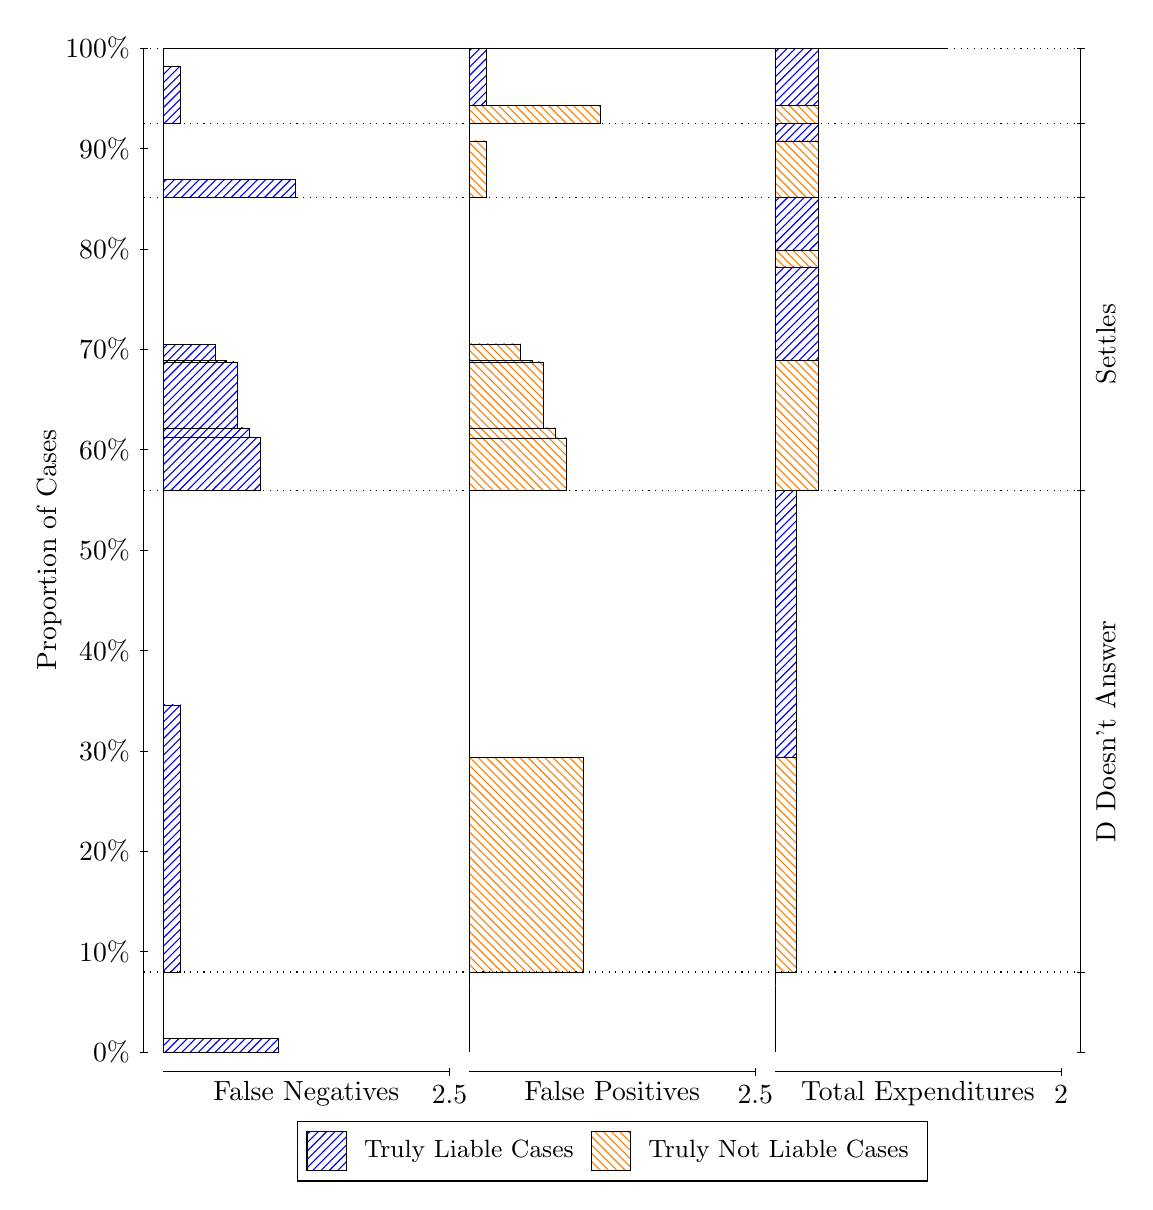
\begin{tikzpicture}
\draw[black, very thin] (1.5,1.75) -- (1.5,14.5);
\node[rotate=90, text=black, anchor=center] at (0.3, 8.125) {Proportion of Cases};
\draw[black, very thin] (1.45,1.75) -- (1.55,1.75);
\node[text=black, anchor=east] at (1.45, 1.75) {0\%};
\draw[black, very thin] (1.45,3.025) -- (1.55,3.025);
\node[text=black, anchor=east] at (1.45, 3.025) {10\%};
\draw[black, very thin] (1.45,4.3) -- (1.55,4.3);
\node[text=black, anchor=east] at (1.45, 4.3) {20\%};
\draw[black, very thin] (1.45,5.575) -- (1.55,5.575);
\node[text=black, anchor=east] at (1.45, 5.575) {30\%};
\draw[black, very thin] (1.45,6.85) -- (1.55,6.85);
\node[text=black, anchor=east] at (1.45, 6.85) {40\%};
\draw[black, very thin] (1.45,8.125) -- (1.55,8.125);
\node[text=black, anchor=east] at (1.45, 8.125) {50\%};
\draw[black, very thin] (1.45,9.4) -- (1.55,9.4);
\node[text=black, anchor=east] at (1.45, 9.4) {60\%};
\draw[black, very thin] (1.45,10.675) -- (1.55,10.675);
\node[text=black, anchor=east] at (1.45, 10.675) {70\%};
\draw[black, very thin] (1.45,11.95) -- (1.55,11.95);
\node[text=black, anchor=east] at (1.45, 11.95) {80\%};
\draw[black, very thin] (1.45,13.225) -- (1.55,13.225);
\node[text=black, anchor=east] at (1.45, 13.225) {90\%};
\draw[black, very thin] (1.45,14.5) -- (1.55,14.5);
\node[text=black, anchor=east] at (1.45, 14.5) {100\%};

\draw[black, very thin] (13.4,1.75) -- (13.4,14.5);
\draw[black, very thin] (13.35,1.75) -- (13.45,1.75);
\node[anchor=west] at (13.35, 1.75) {};
\draw[black, very thin] (13.35,2.7661) -- (13.45,2.7661);
\node[anchor=west] at (13.35, 2.7661) {};
\draw[black, very thin] (13.35,8.8821) -- (13.45,8.8821);
\node[anchor=west] at (13.35, 8.8821) {};
\draw[black, very thin] (13.35,12.601) -- (13.45,12.601);
\node[anchor=west] at (13.35, 12.601) {};
\draw[black, very thin] (13.35,13.547) -- (13.45,13.547);
\node[anchor=west] at (13.35, 13.547) {};
\draw[black, very thin] (13.35,14.493) -- (13.45,14.493);
\node[anchor=west] at (13.35, 14.493) {};
\draw[black, very thin] (13.35,14.497) -- (13.45,14.497);
\node[anchor=west] at (13.35, 14.497) {};
\draw[black, very thin] (13.35,14.5) -- (13.45,14.5);
\node[anchor=west] at (13.35, 14.5) {};

\draw[black, very thin, pattern color=blue, pattern=north east lines] (1.75,1.75) rectangle (3.2033,1.9249);
\draw[black, very thin, pattern color=orange, pattern=north west lines] (1.75,1.9249) rectangle (1.75,2.7661);
\draw[black, very thin, pattern color=blue, pattern=north east lines] (1.75,2.7661) rectangle (1.968,6.1572);
\draw[black, very thin, pattern color=orange, pattern=north west lines] (1.75,6.1572) rectangle (1.75,8.8821);
\draw[black, very thin, pattern color=blue, pattern=north east lines] (1.75,8.8821) rectangle (2.9853,9.5506);
\draw[black, very thin, pattern color=blue, pattern=north east lines] (1.75,9.5506) rectangle (2.84,9.6746);
\draw[black, very thin, pattern color=blue, pattern=north east lines] (1.75,9.6746) rectangle (2.6947,10.515);
\draw[black, very thin, pattern color=blue, pattern=north east lines] (1.75,10.515) rectangle (2.5493,10.529);
\draw[black, very thin, pattern color=blue, pattern=north east lines] (1.75,10.529) rectangle (2.404,10.741);
\draw[black, very thin, pattern color=orange, pattern=north west lines] (1.75,10.741) rectangle (1.75,12.601);
\draw[black, very thin, pattern color=blue, pattern=north east lines] (1.75,12.601) rectangle (3.4213,12.828);
\draw[black, very thin, pattern color=orange, pattern=north west lines] (1.75,12.828) rectangle (1.75,13.547);
\draw[black, very thin, pattern color=blue, pattern=north east lines] (1.75,13.547) rectangle (1.968,14.266);
\draw[black, very thin, pattern color=orange, pattern=north west lines] (1.75,14.266) rectangle (1.75,14.493);
\draw[black, very thin, pattern color=blue, pattern=north east lines] (1.75,14.493) rectangle (5.8193,14.495);
\draw[black, very thin, pattern color=orange, pattern=north west lines] (1.75,14.495) rectangle (1.75,14.497);
\draw[black, very thin, pattern color=orange, pattern=north west lines] (1.75,14.497) rectangle (1.75,14.498);
\draw[black, very thin, pattern color=blue, pattern=north east lines] (1.75,14.498) rectangle (1.75,14.5);
\draw[black, very thin, pattern color=orange, pattern=north west lines] (5.6333,1.75) rectangle (5.6333,2.5912);
\draw[black, very thin, pattern color=blue, pattern=north east lines] (5.6333,2.5912) rectangle (5.6333,2.7661);
\draw[black, very thin, pattern color=orange, pattern=north west lines] (5.6333,2.7661) rectangle (7.0867,5.491);
\draw[black, very thin, pattern color=blue, pattern=north east lines] (5.6333,5.491) rectangle (5.6333,8.8821);
\draw[black, very thin, pattern color=orange, pattern=north west lines] (5.6333,8.8821) rectangle (6.8687,9.5495);
\draw[black, very thin, pattern color=orange, pattern=north west lines] (5.6333,9.5495) rectangle (6.7233,9.6749);
\draw[black, very thin, pattern color=orange, pattern=north west lines] (5.6333,9.6749) rectangle (6.578,10.515);
\draw[black, very thin, pattern color=orange, pattern=north west lines] (5.6333,10.515) rectangle (6.4327,10.53);
\draw[black, very thin, pattern color=orange, pattern=north west lines] (5.6333,10.53) rectangle (6.2873,10.742);
\draw[black, very thin, pattern color=blue, pattern=north east lines] (5.6333,10.742) rectangle (5.6333,12.601);
\draw[black, very thin, pattern color=orange, pattern=north west lines] (5.6333,12.601) rectangle (5.8513,13.32);
\draw[black, very thin, pattern color=blue, pattern=north east lines] (5.6333,13.32) rectangle (5.6333,13.547);
\draw[black, very thin, pattern color=orange, pattern=north west lines] (5.6333,13.547) rectangle (7.3047,13.774);
\draw[black, very thin, pattern color=blue, pattern=north east lines] (5.6333,13.774) rectangle (5.8513,14.493);
\draw[black, very thin, pattern color=orange, pattern=north west lines] (5.6333,14.493) rectangle (5.6333,14.496);
\draw[black, very thin, pattern color=blue, pattern=north east lines] (5.6333,14.496) rectangle (5.6333,14.497);
\draw[black, very thin, pattern color=orange, pattern=north west lines] (5.6333,14.497) rectangle (9.7027,14.498);
\draw[black, very thin, pattern color=blue, pattern=north east lines] (5.6333,14.498) rectangle (8.2493,14.5);
\draw[black, very thin, pattern color=orange, pattern=north west lines] (9.5167,1.75) rectangle (9.5167,2.5912);
\draw[black, very thin, pattern color=blue, pattern=north east lines] (9.5167,2.5912) rectangle (9.5167,2.7661);
\draw[black, very thin, pattern color=orange, pattern=north west lines] (9.5167,2.7661) rectangle (9.7892,5.491);
\draw[black, very thin, pattern color=blue, pattern=north east lines] (9.5167,5.491) rectangle (9.7892,8.8821);
\draw[black, very thin, pattern color=orange, pattern=north west lines] (9.5167,8.8821) rectangle (10.062,10.53);
\draw[black, very thin, pattern color=blue, pattern=north east lines] (9.5167,10.53) rectangle (10.062,11.72);
\draw[black, very thin, pattern color=orange, pattern=north west lines] (9.5167,11.72) rectangle (10.062,11.932);
\draw[black, very thin, pattern color=blue, pattern=north east lines] (9.5167,11.932) rectangle (10.062,12.601);
\draw[black, very thin, pattern color=orange, pattern=north west lines] (9.5167,12.601) rectangle (10.062,13.32);
\draw[black, very thin, pattern color=blue, pattern=north east lines] (9.5167,13.32) rectangle (10.062,13.547);
\draw[black, very thin, pattern color=orange, pattern=north west lines] (9.5167,13.547) rectangle (10.062,13.774);
\draw[black, very thin, pattern color=blue, pattern=north east lines] (9.5167,13.774) rectangle (10.062,14.493);
\draw[black, very thin, pattern color=orange, pattern=north west lines] (9.5167,14.493) rectangle (11.697,14.496);
\draw[black, very thin, pattern color=blue, pattern=north east lines] (9.5167,14.496) rectangle (11.697,14.497);
\draw[black, very thin, pattern color=orange, pattern=north west lines] (9.5167,14.497) rectangle (11.697,14.498);
\draw[black, very thin, pattern color=blue, pattern=north east lines] (9.5167,14.498) rectangle (11.697,14.5);
\draw[black, dotted] (1.5,2.7661) -- (13.4,2.7661);
\draw[black, dotted] (1.5,8.8821) -- (13.4,8.8821);
\draw[black, dotted] (1.5,12.601) -- (13.4,12.601);
\draw[black, dotted] (1.5,13.547) -- (13.4,13.547);
\draw[black, dotted] (1.5,14.493) -- (13.4,14.493);
\draw[black, dotted] (1.5,14.497) -- (13.4,14.497);
\draw[black, very thin] (1.75,1.5) -- (5.3833,1.5);
\node[text=black, anchor=north] at (3.5667, 1.5) {False Negatives};
\draw[black, very thin] (5.3833,1.45) -- (5.3833,1.55);
\node[text=black, anchor=north] at (5.3833, 1.45) {2.5};

\draw[black, very thin] (5.6333,1.5) -- (9.2667,1.5);
\node[text=black, anchor=north] at (7.45, 1.5) {False Positives};
\draw[black, very thin] (9.2667,1.45) -- (9.2667,1.55);
\node[text=black, anchor=north] at (9.2667, 1.45) {2.5};

\draw[black, very thin] (9.5167,1.5) -- (13.15,1.5);
\node[text=black, anchor=north] at (11.333, 1.5) {Total Expenditures};
\draw[black, very thin] (13.15,1.45) -- (13.15,1.55);
\node[text=black, anchor=north] at (13.15, 1.45) {2};


\node[text=black, centered, rotate=90] at (13.72, 5.8241) {D Doesn't Answer};
\node[text=black, centered, rotate=90] at (13.72, 10.741) {Settles};





\draw (7.449999999999999,1.5) node[draw=none] (baseCoordinate) {};
\begin{scope}[align=center]
        \matrix[scale=0.5, draw=black, below=0.5cm of baseCoordinate, nodes={draw}, column sep=0.1cm]{
            \node[rectangle, draw, minimum width=0.5cm, minimum height=0.5cm, pattern color=blue, pattern=north east lines] {}; &
            \node[draw=none, font=\small, text=black] (B) {Truly Liable Cases}; &
            \node[rectangle, draw, minimum width=0.5cm, minimum height=0.5cm, pattern color=orange, pattern=north west lines] {}; &
            \node[draw=none, font=\small, text=black] (B) {Truly Not Liable Cases}; \\
            };
\end{scope}

\end{tikzpicture}
\end{document}